\documentclass{sigchi-ext}
% Please be sure that you have the dependencies (i.e., additional
% LaTeX packages) to compile this example.
\usepackage[T1]{fontenc}
\usepackage{textcomp}
\usepackage[scaled=.92]{helvet} % for proper fonts
\usepackage{graphicx} % for EPS use the graphics package instead
\usepackage{balance}  % for useful for balancing the last columns
\usepackage{booktabs} % for pretty table rules
\usepackage{ccicons}  % for Creative Commons citation icons
\usepackage{ragged2e} % for tighter hyphenation
\usepackage[utf8]{inputenc} % for a UTF8 editor only

\copyrightinfo{Permission to make digital or hard copies of all or
part of this work for personal or classroom use is granted without
fee provided that copies are not made or distributed for profit or
commercial advantage and that copies bear this notice and the full
citation on the first page. Copyrights for components of this work
owned by others than ACM must be honored. Abstracting with credit is
permitted. To copy otherwise, or republish, to post on servers or to
redistribute to lists, requires prior specific permission and/or a
fee. Request permissions from permissions@acm.org.\\
{\emph{CHI'14}}, April 26--May 1, 2014, Toronto, Canada. \\
Copyright \copyright~2014 ACM ISBN/14/04...\$15.00. \\
DOI string from ACM form confirmation}

% Paper metadata (use plain text, for PDF inclusion and later
% re-using, if desired).  Use \emtpyauthor when submitting for review
% so you remain anonymous.
\def\plaintitle{Emotion-based music recommendation using supervised learning}
\def\plainauthor{Karl-Arnold Bodarwé, Philipp Jean-Jacques, Jenny Noack}
\def\emptyauthor{}
\def\plainkeywords{music recommendation;music emotion;supervised learning;naive bayes;mfcc;rms;chroma;}
\def\plaingeneralterms{Music Recommendation}

\title{Emotion-based music recommendation using supervised learning}

\numberofauthors{3}
% Notice how author names are alternately typesetted to appear ordered
% in 2-column format; i.e., the first 4 autors on the first column and
% the other 4 auhors on the second column. Actually, it's up to you to
% strictly adhere to this author notation.
\author{%
  \alignauthor{%
    \textbf{Karl-Arnold Bodarwé}\\
    \affaddr{University of Regensburg} \\
    \affaddr{Regensburg, Bayern, 93053, Germany} \\
    \affaddr{karl-arnold.bodarwe@stud.uni-regensburg.de} }\alignauthor{%
    \textbf{Jenny Noack}\\
    \affaddr{University of Regensburg} \\
    \affaddr{Regensburg, Bayern, 93053, Germany} \\
    \affaddr{jenny.noack@stud.uni-regensburg.de} } \vfil \alignauthor{%
    \textbf{Philipp Jean-Jacques}\\
    \affaddr{University of Regensburg} \\
    \affaddr{Regensburg, Bayern, 93053, Germany} \\
    \affaddr{philipp.jean-jacques@stud.uni-regensburg.de} }\alignauthor{%
  }
}
% Make sure hyperref comes last of your loaded packages, to give it a
% fighting chance of not being over-written, since its job is to
% redefine many LaTeX commands.
\definecolor{linkColor}{RGB}{6,125,233}
\hypersetup{%
  pdftitle={\plaintitle},
  pdfauthor={\plainauthor},
  pdfkeywords={\plainkeywords},
  bookmarksnumbered,
  pdfstartview={FitH},
  colorlinks,
  citecolor=black,
  filecolor=black,
  linkcolor=black,
  urlcolor=linkColor,
  breaklinks=true,
}

\begin{document}

\maketitle

% Uncomment to disable hyphenation (not recommended)
% https://twitter.com/anjirokhan/status/546046683331973120
\RaggedRight{}

\begin{abstract}
Music recommendation systems are well explored and commonly used but are normally based on
manually tagged parameters and simple similarity calculation. Our project proposes a recommendation system based on emotional computing, automatic classification and feature extraction, which recommends music based on the emotion expressed by the song.\\
To achieve this goal a set of features is extracted from the song, including the MFCC (mel-frequency cepstral coefficients) following the works of McKinney et al. \cite{Mckinney2003} and a machine learning system is trained on a set of 424 songs, which are categorized by emotion. The categorization of the song is performed manually by multiple persons to avoid error. The emotional categorization is performed using a modified version of the Tellegen-Watson-Clark emotion model \cite{Tellegen1999}, as proposed by Trohidis et al. \cite{Trohidis2011}.
The System is intended as desktop application that can reliably determine similarities between the main emotion in multiple pieces of music, allowing the user to choose music by emotion. We report our findings below.
\end{abstract}

\keywords{\plainkeywords}

\category{H.3.2}{Record classification}{Miscellaneous}

\section{Introduction}
Music recommendation systems are well known and widespread. Using methods such as tags or similar user behaviour, pieces of music can be recommended by a variety of features.\\
Music and emotion are strongly related to each other \cite{Krumhansl2002} but emotion is rarely considered in existing recommendation systems. In our approach we implemented a system that recommends music by emotion. The emotion of the song is determined using a classifier that is trained on audio-features extracted from the song. The extracted emotion is then used to recommend a song to the user.

\section{Related Work}
The key problem in our recommendation system was to classify music by its emotion. There have been various approaches in classifying music and audio in general such as \cite{Mckinney2003,Cook2007,Jeremic2015,Tzanetakis2002}, with an accuracy up to 74\%. Though the results of these approaches are very promising, classifying music by emotion yields worse results \cite{Kim2010}. There have also been various approaches on how to classify a piece of music by its emotion. They utilize different emotion models, as well as different feature extraction techniques. Most of them use versions of either the \textit{Tellegen-Watson-Clark-Model} \cite{Trohidis2011} or the \textit{Valence-Arousal-Model} \cite{Kim2011}. \cite{Kim2010} shows, that a set of timbral features such as MFCC and RMS provide a solid set of features for emotion classification.

\begin{marginfigure}[0pc]
  \begin{minipage}{\marginparwidth}
    \centering
    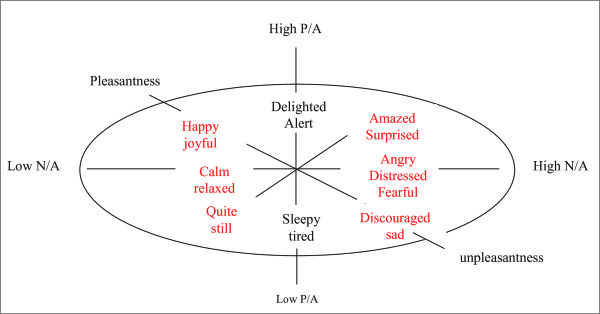
\includegraphics[width=1.0\marginparwidth]{images/tellegen-watson-clark-model.png}
    \caption{Tellegen-Watson-Clark model of mood \cite{Tellegen1999}}~\label{fig:tellegen-watson-clark}
  \end{minipage}
\end{marginfigure}

\section{Emotion Model}\label{sec:emotion-model}
The Tellegen-Watson-Clark model, as used by \cite{Trohidis2011} has two axes labeled Positive Affect and Negative Affect which map emotions accordingly. Another dimension that can be derived from this model is the level of pleasantness of a certain emotion.\\
To be able to distinguish between emotions more easily, we decided to use a simplified version of the Tellegen-Watson-Clark model. We defined four emotional categories, marking the extreme ends of the graphs used in the model. The categories proposed in the Tellegen-Watson-Clark model have some adjectives that are very similar and difficult to distinguish especially when dealing with music as a carrier of emotion. Categories such as \textit{calm-relaxing} and \textit{quiet-still}, or \textit{amazed-surprised} and \textit{happy-pleased} were combined into one category. The remaining categories are:

\begin{itemize}
	\item calm-relaxing
	\item happy-amazed
	\item angry-fearful
	\item sad-lonely
\end{itemize}

\section{Training Data}\label{training-data}
To create the training data for the classifier, we accumulated a collection of 424 songs of various genre and artist. To achieve a preferably even distribution over the four emotion categories described above, we searched various online streaming and video platforms, such as YouTube and Spotify, for playlists with tags fitting our categories, such as \textit{angry, sad, relaxing} or \textit{happy}.\\
Those songs were then tagged by three independent raters into the four emotional categories mentioned above. Afterwards \textit{Fleiss' Kappa} was calculated over the results, to use only songs for the creation of the training data where all raters agreed on the same emotion. The following table shows the distribution of kappa values over all songs.\\

\begin{table}
  \centering
  \label{fig:kappa-distribution}
  \begin{tabular}{@{}lll@{}}
    Kappa & Count & Percent \\ \midrule
    1.00 & 260 & 61.32\% \\
    0.33 & 155 & 36.56\% \\
    0.00 & 9 	 & 2.12\%
  \end{tabular}
  \caption{Distribution of Kappa values across tagged values}
\end{table}

Most of the disagreement (90 songs) were in categories \textit{calm-relaxing} and \textit{sad-lonely}, predicting difficulties in the differentiation of these categories.\\

\begin{marginfigure}[0pc]
  \begin{minipage}{\marginparwidth}
    \centering
    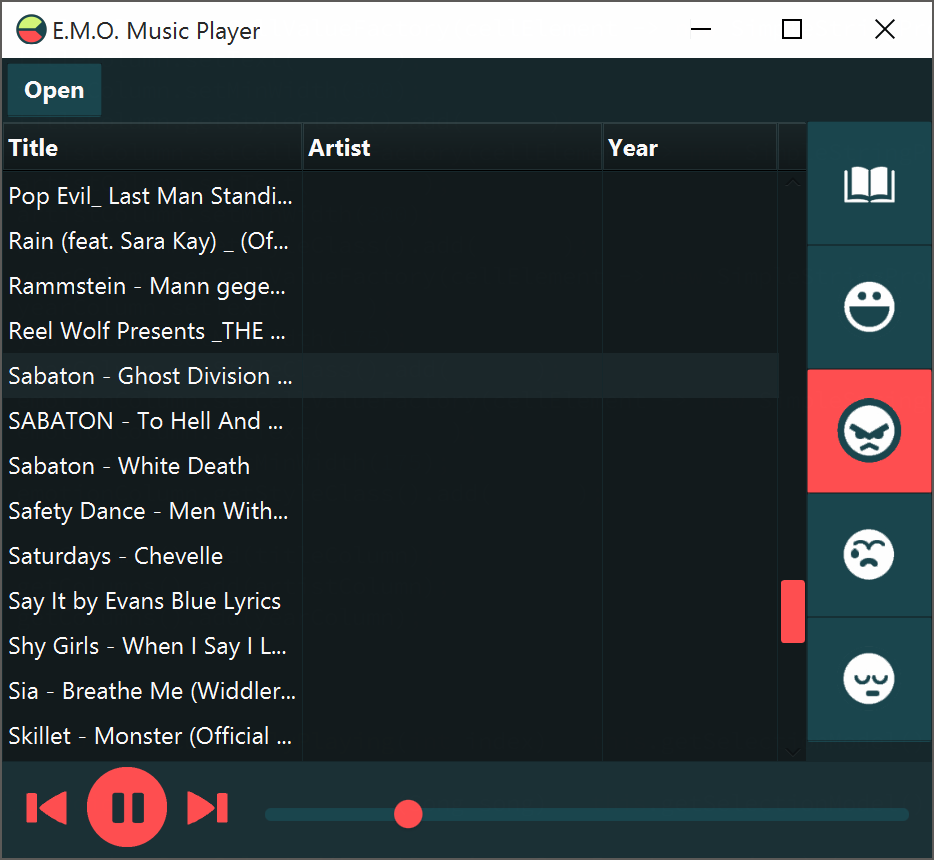
\includegraphics[width=1.0\marginparwidth]{images/screenshot.png}
  	\caption{User interface of the music player}~\label{fig:screenshot}
  \end{minipage}
\end{marginfigure}

\section{Feature extraction and classification}\label{sec:feature-extraction}
Previous research on which features to use for audio classification has shown that MFCC, along with several low level features, such as RMS, show promising results \cite{Trohidis2011,Kim2010}. We decided to use these features, along with the \textit{Chroma}-feature for our classification. Because the application is meant to be used in real time, the feature extraction needs to be as fast as possible. Therefore as few features as possible were used without impairing the accuracy of the classification too much. The final feature vector consists of 26 features.

\begin{table}
  \centering
  \begin{tabular}{@{}ll@{}}
    Feature Count & Feature Name \\ \midrule
    13 & MFCC \\
    12 & Chroma \\
    1  & RMS
  \end{tabular}
  \caption{Feature vector}
  \label{feature-vector}
\end{table}

The audio processing library we used was \textit{jAudio} \cite{McEnnis2005}, a gui application specifically developed for feature extraction which supports both wav and mp3 formats. The classification is done by a Naive Bayes classifier, because it showed the best performance in comparison to the other classifiers tested (Support Vector Machine, Logistic Regression, Decision Trees).

\section{Recommendation System}
The system was implemented as a simple music player. A song is classified as soon as it is loaded into the music library of the player, using the technique mentioned above. The system provides recommendations based on the users selection of emotion. Therefore the user interface provides a set of buttons associated with the emotion categories (angry, sad, calm, happy), which allow the user to select the desired music emotion. The system displays the resulting recommendations as a playlist.

\section{Results}
The emotion of a song is a highly subjective experience, given that only 61.32\% of the songs were tagged with the same label. The classifier was trained using the data explained in the \textit{training data} section and was evaluated using 10-fold cross validation. The classification yields an accuracy of 53.07\%. Similar approaches as reviewed by \cite{Kim2010} achieve accuracies ranging from 45\% to 65\%. Better results were only achieved when using more features or additional information such as the lyrics. An informal test of the recommendation system with five users showed, that they were not disappointed by the performance of the system.

\begin{table}
  \centering
  \begin{tabular}{@{}lll@{}}
    Correctly Classified          & 138       & 53.07\% \\
    Incorrectly Classified        & 122       & 46.93\% \\
    Kappa statistic               & 0.35      & \\
    Mean absolute error           & 0.23      & \\
    Root mean squared error       & 0.45      & \\
    Relative absolute error       & 64.52\%   & \\
    Root relative squared error   & 105.10\%  & \\
    Total Number of Instances     & 260       & 100\%
  \end{tabular}
  \caption{Evaluation of the Naive Bayes classifier}
\end{table}

\section{Conclusion}
We found that it is possible to classify music via emotion and built a recommendation system around that classification. A recommendation system such as this could be improved by recommending music based on the correlation between user emotion or user behaviour and music emotion.\\
With the refinement of the extracted features, we are positive that the accuracy of the classification can be improved. Additional features would take even longer to extract from a song. As mentioned above the used features were specifically chosen to make sure that the feature extraction process was as fast as possible, to provide the best possible user experience when using the recommendation system.

\bibliographystyle{SIGCHI-Reference-Format}
\bibliography{literature}

\end{document}
